\documentclass[a4paper,english,helvetica,nologo,openbib,totpages]{europecv}
\usepackage[english]{babel} % This is mandatory
\usepackage[margin=1cm]{geometry}
\usepackage[hidelinks,unicode]{hyperref}
\usepackage{graphicx}
\usepackage{enumitem}

\makeatletter%
\renewcommand*\ecvtitle{%taken from definition file ecven.def and adapted to requirement
    \ecv@utf{\Large\textbf{C\ecv@kern u\ecv@kern r\ecv@kern r\ecv@kern
            i\ecv@kern c\ecv@kern u\ecv@kern l\ecv@kern u\ecv@kern m \ecv@kern V\ecv@kern
            i\ecv@kern t\ecv@kern a\ecv@kern e}}
}

\begin{document}

\pagestyle{empty}

% picture
\begin{minipage}{\textwidth}
	\raggedleft
    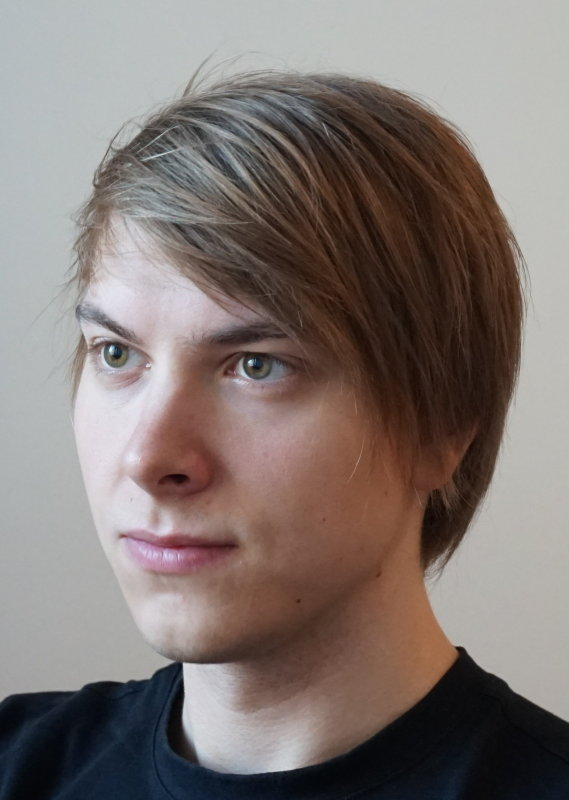
\includegraphics[height=7cm]{photo.jpg}
\end{minipage}
\vspace{-7.6cm}

\begin{europecv}

\vspace{0.5cm}

\ecvsection{Personal Information}
\ecvitem[5pt]{First name / Surname}{Tomáš Křížek}
\ecvitem[5pt]{Telephone}{+420 xxx xxx xxx}
\ecvitem[5pt]{E-mail}{\href{mailto:tomas.krizek@mailbox.org}{tomas.krizek@mailbox.org}}
\ecvitem[5pt]{Date of birth}{dd. mm. yyyy}
\ecvitem[5pt]{Permanent Address}{perm address}
\ecvitem[5pt]{GitHub}{\url{https://github.com/tomaskrizek}}


\ecvsection{Experience}

\ecvitem{2018--present}{
\textbf{Research Software Engineer}\newline
\textit{CZ.NIC}
\begin{itemize}
  \item Working with low-level network protocols -- DNS, TLS, HTTP.
  \item Design \& development of DNS testing and benchmarking tools.
  \item Development of DNS resolver \& DNS-over-HTTPS functionality.
  \item Automation of CI testing \& maintenance of 10+ servers.
  \item Packaging software for Linux distributions (rpm, deb).
\end{itemize}
\textit{Python, C, Lua, Rust, git, DNS, Linux, Ansible, Bash, Docker}
\newline}

\ecvitem{2016--2017}{
\textbf{Associate Software Engineer}\newline
\textit{Red Hat}
\begin{itemize}
  \item Development of identity management solution.
  \item Design \& development of test automation framework.
  \item Packaging software for Linux distributions (rpm).
\end{itemize}
\textit{Python, Linux, git, Ansible, Bash, Docker, DNS}
\newline}

\ecvitem{2015--2016}{
\textbf{Python Developer}\newline
\textit{Technical University of Liberec}
\begin{itemize}
  \item Design \& development of multi-platform desktop application.
\end{itemize}
\textit{Python, git, Linux}
\newline}


\ecvsection{Education}

\ecvitem[8pt]
{2014--2016}{
\textbf{Master's degree}, Information Technology \textit{(cum laude)}\newline
Technical University of Liberec, Czech Republic}

\ecvitem[8pt]
{2011--2014}{
\textbf{Bachelor's degree}, Information Technology \textit{(cum laude)}\newline
Technical University of Liberec, Czech Republic}


\ecvsection{Skills}
\ecvitem{Python}{advanced}
\ecvitem{Linux}{advanced}
\ecvitem{Ansible}{advanced}
\ecvitem{Bash}{intermediate}


\ecvsection{Skills}
\ecvitem{Python}{advanced}
\ecvitem{Linux}{advanced}
\ecvitem{Ansible}{advanced}
\ecvitem{Bash}{intermediate}


\ecvsection{Certificates}
\ecvitem[6pt]{Ansible}{
Expertise in Ansible Automation\newline
\textit{Red Hat}}
\ecvitem[6pt]{CCNA Exploration}{
CCNA Exploration: Network Fundamentals\newline
\textit{Cisco Networking Academy}}
\ecvitem[6pt]{IT Essentials}{
IT Essentials: PC Hardware and Software\newline
\textit{Cisco Networking Academy}}


\end{europecv}

\end{document}
